Go is a board game noted for its simple rules but many-layered complexity. Go is played by two players, Black and White, who consecutively place a stone of their colour on an empty intersection of a square grid. Black starts first. The standard board size is 19×19, but 9×9 and 13×13 are also played. A \textit{group} is a connected set of stones (using 4-connectivity) of the same color (cf. Fig.~\ref{Go_1}). \textit{Liberties} are empty locations surrounding a group. A group is captured when it has no more liberties. The stones of a group are removed from the board once captured. It is illegal to play moves that would result in self-capture. A \textit{group} is termed \textit{dead} when it is inevitable that it will be captured. The \textit{objective} of the game is to secure more territory than the other player. The game ends when both players pass. Each player gets one point for every location of territory that they captured and one point for each captured stone. In addition, white receives a bonus, known as \textit{komi}, compensating for black played first. The player with the highest score wins. According to regional rules, the precise scoring details vary; however, all major scoring systems almost always lead to the same result. More rules on \textit{handicap}, \textit{Ko}, \textit{life and death}, and others are well described in\cite{b11,b14,b15} (cf. Fig.~\ref{Go_1}, shows a game of 19 × 19).
% A \textit{handicap} is the number of compensation stones that the black player is allowed to place on the board before alternating play. It allows players of different strengths to play competitively. `Even games' are games with \textit{handicap} $0$ and a \textit{komi} of $7.5$ (the \textit{komi} can vary according to regional rules). 
The ranks of amateur Go players are ordered by decreasing \textit{kyu} and then increasing \textit{dan}, where the difference in rank corresponds to the number of handicap stones required to maintain parity. Professional players are ordered by increasing \textit{dan} on a second scale (cf. Fig.~\ref{Go_ranking}). The title `top professional' is given to a professional player who has recently won at least one major tournament.
\begin{figure}[b]
    \centering
    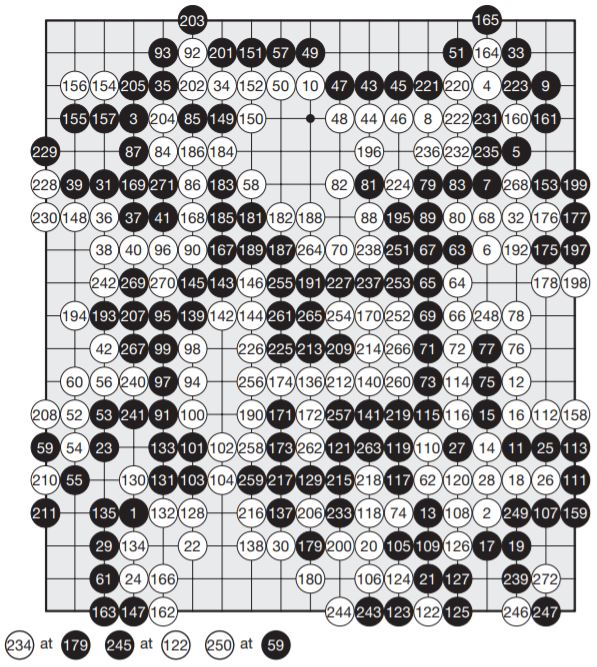
\includegraphics[width = 0.6\columnwidth]{Go_3}
    \caption{Fan Hui (Black), AlphaGo (White), AlphaGo wins by 2.5 points\cite{b12}}
    \label{Go_1}
\end{figure}

Combinatorial games have several ways of measuring game complexity,\cite{b3,b16}. Most widely used are \textit{state-space} complexity and \textit{game-tree} complexity (our main focus). The state-space complexity is defined as the number of legal game positions reachable from the initial position of the game. Whereas game-tree complexity is the total number of possible games that can be played; the total number of all possible reachable leaf nodes (end of the game) from the game's root node (initial position). Game-tree complexity may be larger than the state-space complexity, as the same position may occur at several different places in the game tree. Calculating the exact game-tree complexity of games such as chess is infeasible. Therefore, using tournament games, we observe the average game length, i.e., depth $d$, and determine the average branching factor $b$, either as a constant or a function of depth. Finally, raising the average branching factor $b$ to the power of the average length $d$, i.e., $b^d$, gives us an approximation. So, in large games, such as chess, we have $b \approx 35$ and $d \approx 80$, and Go has $b \approx 250$ and $d \approx 150$\cite{b4}. Thus an enormous game-tree complexity of $250^{150}$ (more than the number of atoms in the universe) for Go is intractable using brute force approaches.

\begin{figure}[t]
    \centering
    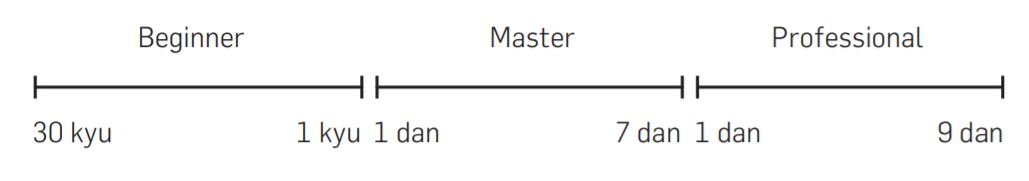
\includegraphics[width = \columnwidth]{Go_2}
    \caption{Ranking system in the game of Go\cite{b11}}
    \label{Go_ranking}
\end{figure}